\hypertarget{ppE__IMRPhenomD_8cpp}{}\section{src/pp\+E\+\_\+\+I\+M\+R\+PhenomD.cpp File Reference}
\label{ppE__IMRPhenomD_8cpp}\index{src/pp\+E\+\_\+\+I\+M\+R\+Phenom\+D.\+cpp@{src/pp\+E\+\_\+\+I\+M\+R\+Phenom\+D.\+cpp}}
{\ttfamily \#include \char`\"{}pp\+E\+\_\+\+I\+M\+R\+Phenom\+D.\+h\char`\"{}}\newline
{\ttfamily \#include $<$math.\+h$>$}\newline
{\ttfamily \#include $<$adolc/adouble.\+h$>$}\newline
{\ttfamily \#include $<$adolc/taping.\+h$>$}\newline
{\ttfamily \#include $<$adolc/drivers/drivers.\+h$>$}\newline
{\ttfamily \#include $<$iostream$>$}\newline
{\ttfamily \#include $<$cmath$>$}\newline
{\ttfamily \#include $<$complex$>$}\newline
{\ttfamily \#include \char`\"{}util.\+h\char`\"{}}\newline
Include dependency graph for pp\+E\+\_\+\+I\+M\+R\+Phenom\+D.\+cpp\+:\nopagebreak
\begin{figure}[H]
\begin{center}
\leavevmode
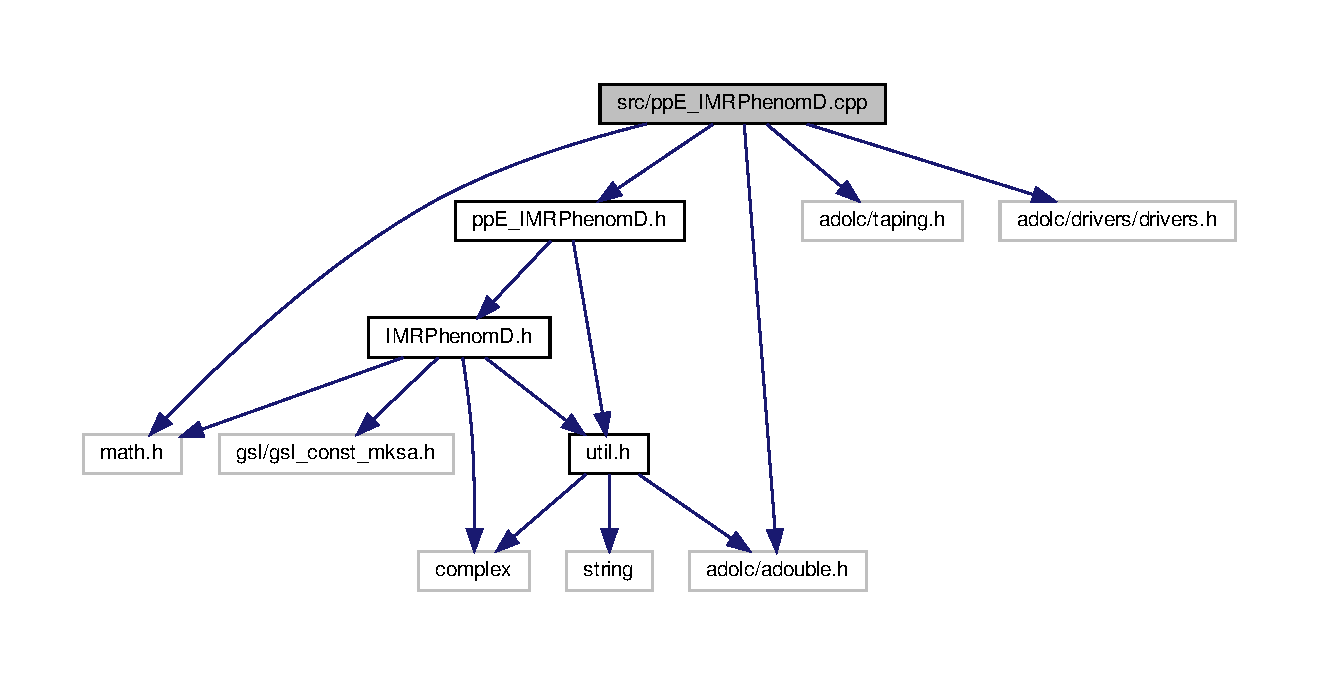
\includegraphics[width=350pt]{ppE__IMRPhenomD_8cpp__incl}
\end{center}
\end{figure}


\subsection{Detailed Description}
File for the implementation of the ppE formalism for testing GR

Extends the \hyperlink{classIMRPhenomD}{I\+M\+R\+PhenomD} template to include non-\/\+GR phase terms

Supported waveforms\+: ppE Inspiral, ppE I\+MR, d\+CS, Ed\+GB 